\documentclass[journal]{new-aiaa}

\usepackage[utf8]{inputenc}
\usepackage{textcomp}
\usepackage{graphicx}
\usepackage{amsmath}
\usepackage{siunitx}
\usepackage{booktabs}
\usepackage{url}
\usepackage{xcolor}
\hypersetup{hidelinks}
\graphicspath{{figures/}}

\title{Adaptive Physics-Informed Thermal Digital Twins:\\PINN and Streamed-PINO Models for Rocket-Wall Heat Conduction}

\author{Gabriel Berezovsky}
\affil{gabrielb@campus.technion.ac.il, 941220121}
\author{Joshua Blecher}
\affil{bjoshua@campus.technion.ac.il, 941220097}
\author{Nathan Florsheim}
\affil{nathanf@campus.technion.ac.il, 800001653}

\begin{document}
\maketitle

\begin{abstract}
This work develops a causal thermal digital twin for a regeneratively cooled rocket-throat wall using physics-informed neural networks (PINNs) and a streamed physics-informed neural operator (PINO). A one-dimensional through-thickness prototype first verifies the governing physics, reference solver, and sensor-assimilation pipeline. Training stability is then evaluated using five seeds, a fixed analytical corpus, and a locked heat-flux step. Mean overall RMSE is $19.502\pm1.441$ K for the offline PINN, $2.208\pm0.375$ K for the sensor-adaptive PINN, and $0.2327\pm0.0060$ K for the streamed PINO (mean $\pm$ sample standard deviation). Adaptation improves on the offline model by a factor of 8.83, while PINO improves on the adaptive model by a further factor of 9.49. PINO post-switch RMSE is $0.2364\pm0.0157$ K and mean median inference latency is $0.862\pm0.085$ ms, compared with $2465\pm152$ ms for an adaptive PINN update. The accuracy and latency advantage is therefore stable across network initialization.
\end{abstract}

\section{Introduction}
Thermal protection and regenerative cooling depend on estimating temperatures at locations where instrumentation is sparse or impractical. A digital twin can combine a governing heat-transfer model with wall measurements to reconstruct the complete temperature field. Classical numerical solvers offer reliable predictions when geometry, properties, and boundary conditions are known, whereas purely data-driven surrogates can update quickly but may extrapolate unphysically. PINNs embed the governing differential equation into the training objective and thereby offer a continuous field representation constrained by physics \cite{raissi2019,cai2021}.

The central question was not simply whether a PINN can solve a heat equation, but whether a thermal model can incorporate sparse measurements when operation changes. Two causal strategies are compared. The adaptive PINN continues optimization using a rolling observation window. The streamed PINO learns a family of heat-solution operators offline; after deployment its weights are fixed and only a recurrent state is updated. Both are evaluated using only measurements available at the current time.

The 1D and 2D studies are a verification hierarchy for the same conduction physics, not unrelated applications. The 1D coordinate resolves wall thickness; the second coordinate resolves in-plane or circumferential variation. The Cartesian square benchmark supplies a separable analytical reference from Hsu, Tu, and Chang \cite{hsu2023}, while the wall model retains dimensional heat flux, convection, and temperature. The source and reproducibility instructions are available in the project repository \cite{repository}.

\section{Physical Problem Definition}
\subsection{One-dimensional rocket-wall prototype}
The prototype represents conduction through a wall of thickness $L$. The hot surface at $x=0$ receives a prescribed heat flux and the coolant surface at $x=L$ obeys a convective condition:
\begin{align}
\rho c_p T_t &= kT_{xx},\qquad 0<x<L,\;0<t<t_f, \\
-kT_x(0,t)&=q_{\mathrm{hot}}(t), \\
-kT_x(L,t)&=h_{\mathrm{cool}}[T(L,t)-T_{\mathrm{cool}}],\\
T(x,0)&=T_0 .
\end{align}
Constant copper-like properties and no volumetric generation are assumed. A Crank--Nicolson solution and, in the final physical study, a Robin eigenfunction expansion supply synthetic ground truth. The 1D equation is the locally planar, through-thickness reduction of the wall problem. For an axisymmetric cylindrical wall the radial term is $r^{-1}\partial_r(r\partial_rT)$; over a thin wall with $L/R\ll1$, $r$ varies weakly and curvature enters as a nearly constant geometric correction. The 2D Cartesian benchmark adds a tangential coordinate while retaining the same parabolic diffusion operator.

\begin{figure}[t]
  \centering
  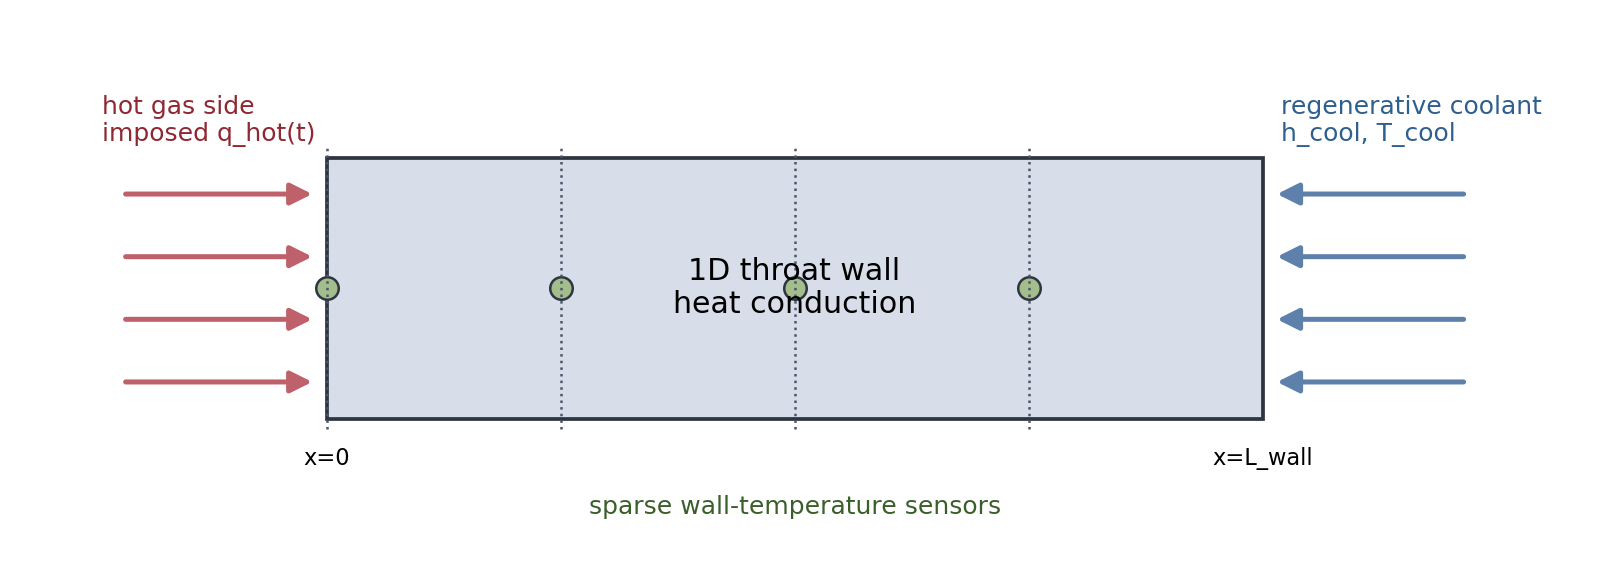
\includegraphics[width=\linewidth]{physical_setup.png}
  \caption{Unified wall interpretation. The 1D model resolves through-thickness conduction; the extended model additionally resolves variation along the wall. Sensors are observation constraints, not boundaries.}
  \label{fig:oneD}
\end{figure}

\subsection{Two-dimensional analytical benchmark}
The extended study uses the dimensionless heat equation on a unit square,
\begin{equation}
 \theta_{\tau}=L_r^2\theta_{XX}+\theta_{YY},\qquad (X,Y)\in(0,1)^2,
 \label{eq:heat2d}
\end{equation}
with $L_r=1$. For literature verification, the four edges have parabolic spatial profiles and independent exponential decay rates:
\begin{align}
\theta(0,Y,\tau)&=(Y-Y^2)e^{-d_1\tau}, &
\theta(1,Y,\tau)&=(Y-Y^2)e^{-d_2\tau},\nonumber\\
\theta(X,0,\tau)&=(X-X^2)e^{-d_3\tau}, &
\theta(X,1,\tau)&=(X-X^2)e^{-d_4\tau},
\end{align}
with $\theta(X,Y,0)=(X-X^2)+(Y-Y^2)$. The analytical solution is evaluated by shifting the nonhomogeneous boundaries and expanding the homogeneous remainder in sine eigenfunctions \cite{hsu2023}.

The adaptive experiment instead applies continuous left-edge heating $\theta(0,Y,\tau)=Y(1-Y)$ and zero temperature on the other edges. At $\tau_s=50$, the heating amplitude rises by 50\%. The event is excluded from the PINN boundary definition, so only subsequently revealed measurements communicate the disturbance. The analytical switch solution preserves the pre-event interior field through a homogeneous sine-series correction while enforcing the new edge values.

\section{Methodology}
\subsection{PINN formulation and verification ladder}
The network maps normalized coordinates to temperature. Automatic differentiation supplies the derivatives in Eq.~\eqref{eq:heat2d}. The offline objective is
\begin{equation}
\mathcal{L}_{0}=w_f\mathcal{L}_{f}+w_b\mathcal{L}_{b}+w_i\mathcal{L}_{i},
\end{equation}
where the three mean-square terms penalize the PDE residual, boundary conditions, and initial condition. The adaptive objective adds sparse observations,
\begin{equation}
\mathcal{L}_{\mathrm{ad}}=\mathcal{L}_{0}+w_d\frac{1}{N_s}
\sum_{j=1}^{N_s}\left[\theta_{\mathrm{PINN}}(\mathbf{x}_j,\tau_j)-\theta_j\right]^2.
\end{equation}

Verification is deliberately layered. Unit tests cover the analytical solution, architecture configuration, batching, metrics, and boundary-switch solver. The 1D neural prediction is checked against Crank--Nicolson. The 2D analytical evaluator is checked against the three tables of Ref.~\cite{hsu2023}. Table 1 is reproduced closely; direct use of the printed equations does not reproduce printed Tables 2 and 3, so only Table 1 is treated as a verified benchmark. Finally, every DeepXDE run stores the resolved TOML configuration beside its metrics and figures.

\subsection{Causal online assimilation}
After offline training, sensor values are revealed in chronological batches. Immediately before assimilation, the current model predicts the newly available points and full analytical field. Those predictions define the causal-prior error. The observations in a recent-history window are then attached as point constraints, and Adam continues from the current weights for a fixed iteration budget. Re-evaluation defines the causal-posterior error. This distinction prevents a final network from being evaluated retrospectively and misrepresented as an online forecast.

The final benchmark uses the same locked analytical heat-flux-step case and corpus for every seed. The PINN has three 48-neuron tanh layers, 2,500 offline Adam iterations, and 381 iterations per adaptive batch. Three wall sensors are sampled in two-instance batches with two recent batches retained. Seeds 7, 11, 19, 23, and 31 alter initialization and training randomness; the corpus remains fixed at data seed 8128. Table~\ref{tab:config} summarizes the matched study.

\subsection{Streamed physics-informed neural operator}
Unlike an instance-specific PINN, an operator network learns a mapping over a family of boundary histories \cite{li2021pino}. The streamed PINO passes three current sensor temperatures, heat flux and its increment, time, and time step through a 96-state GRU. A 96-mode spatial decoder reconstructs temperature from that state and five Fourier coordinate features. Training minimizes field error plus weighted PDE and boundary residuals, with additional emphasis around flux transitions. The fixed corpus contains 600 training, 100 validation, and 200 interpolation-test histories, plus one locked switch case. At deployment, weights are fixed and only the 96-value state evolves; no future or full-field test values enter the online API.

\begin{table}[t]
\caption{Controlled five-seed benchmark configuration.}
\label{tab:config}
\centering
\begin{tabular}{lcc}
\toprule
Setting & Adaptive PINN & Streamed PINO\\
\midrule
Architecture & $48\times3$ tanh & GRU-96, 96 modes\\
Offline training & 2500 iterations & $\leq500$ epochs\\
Online operation & 381 Adam steps/batch & one recurrent step\\
Wall sensors & 3 & 3\\
History & 2 recent batches & 96-value state\\
Study seeds & \multicolumn{2}{c}{7, 11, 19, 23, 31}\\
\bottomrule
\end{tabular}
\end{table}

\section{Results and Discussion}
\subsection{Prototype verification}
The PyTorch prototype establishes that the implementation satisfies the intended heat equation, boundary conditions, nondimensionalization, and streaming-data path. Its Crank--Nicolson reference was separately checked against the constant-flux analytical steady state, agreeing within 0.007 K. Preliminary short-budget runs exposed a cold bias near the flux boundary and motivated the converged DeepXDE configuration used below; they are treated as development diagnostics rather than final performance evidence.

\begin{figure}[t]
  \centering
  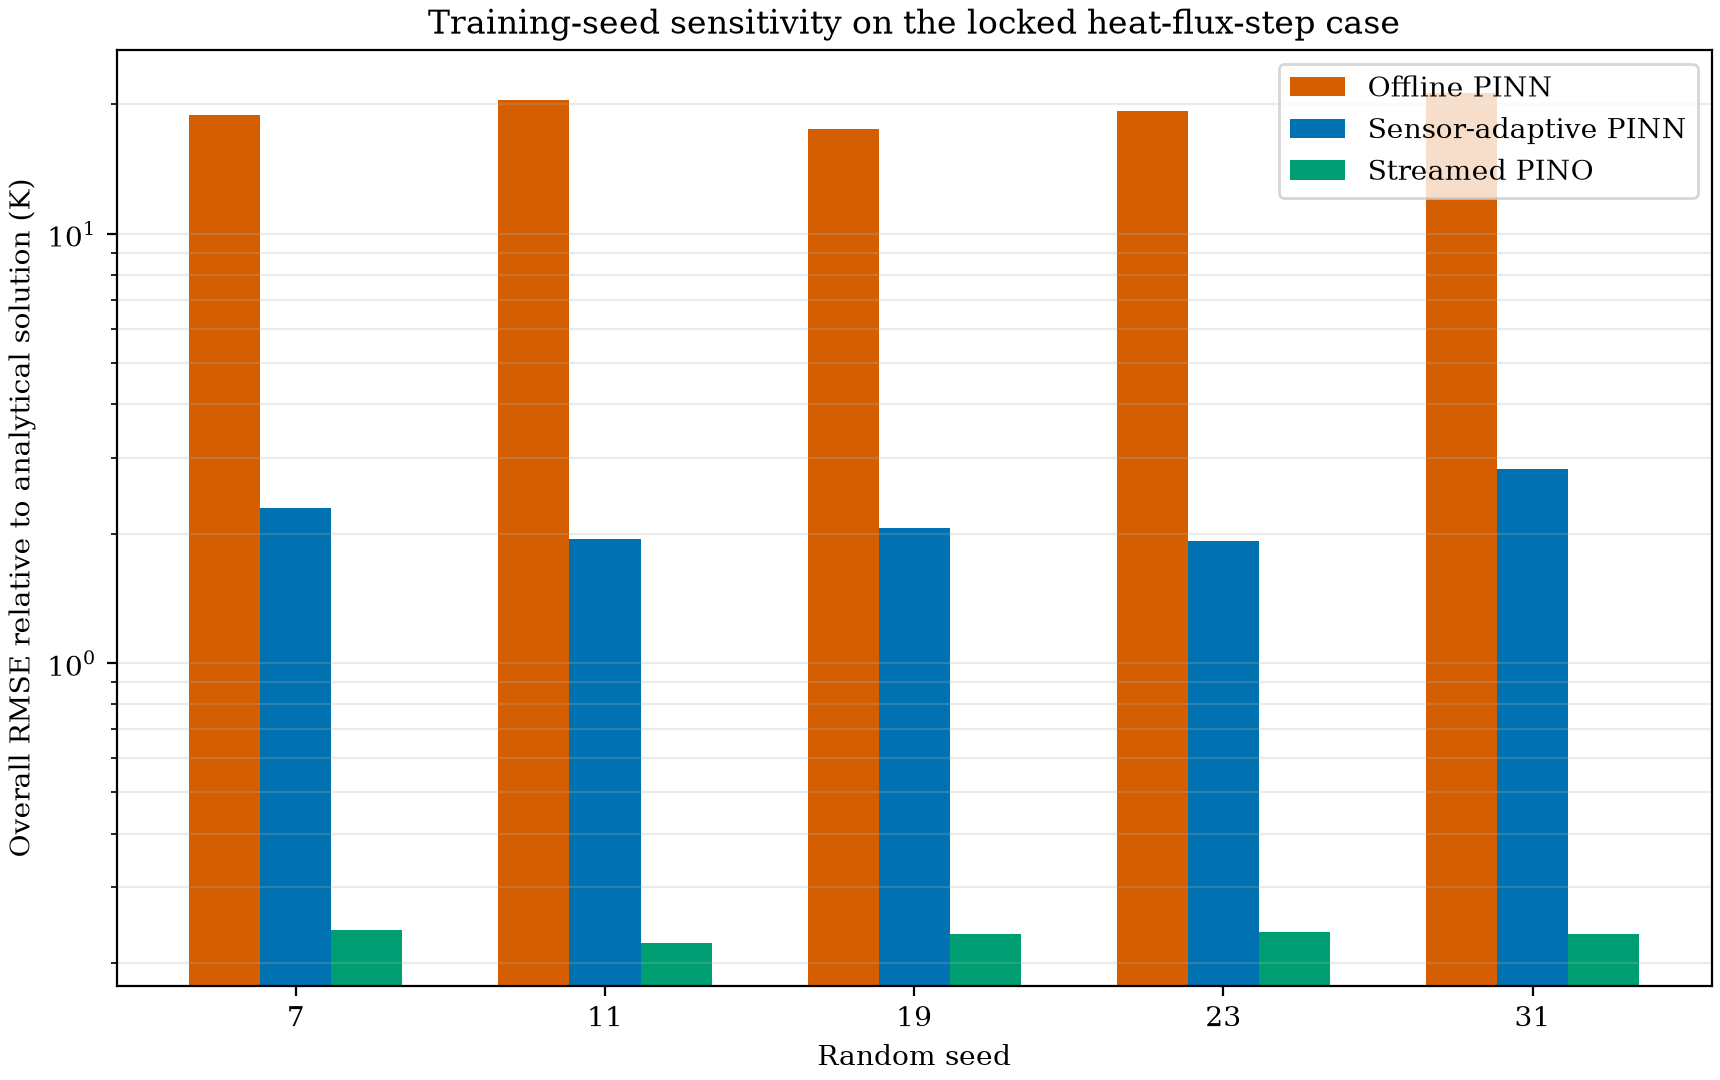
\includegraphics[width=\linewidth]{seedwise_locked_case_rmse.png}
  \caption{Overall locked-case RMSE for every training seed. The logarithmic scale shows consistent separation among offline PINN, adaptive PINN, and streamed PINO.}
  \label{fig:oneDresults}
\end{figure}

\subsection{Five-seed training stability}
Across five seeds, offline PINN overall RMSE is $19.502\pm1.441$ K, whereas adaptive PINN RMSE is $2.208\pm0.375$ K. Their respective ranges are 17.554--21.271 K and 1.921--2.825 K; every adaptive run therefore outperforms every offline run. Post-switch adaptive RMSE is especially stable at $0.4519\pm0.0156$ K (coefficient of variation 3.46\%), although maximum-time RMSE varies more strongly at $8.207\pm1.729$ K. The adaptive benefit is consequently not an artifact of one favorable initialization.

\subsection{Unannounced heat-flux change and PINO comparison}
The locked digital-twin test applies 4.0 MW/m$^2$ followed by an unannounced increase to 5.2 MW/m$^2$ at $t=0.5$ s. Table~\ref{tab:results} reports five-seed mean $\pm$ sample standard deviation. Adaptive assimilation reduces mean overall RMSE by 88.7\%; streamed PINO reduces it by 98.8\% relative to the offline PINN. PINO is also stable across initialization: overall RMSE has a 2.60\% coefficient of variation, and mean RMSE over 200 held-out interpolation histories is $0.2495\pm0.0061$ K across training seeds.

\begin{table}[t]
\caption{Five-seed locked heat-flux-step performance (mean $\pm$ sample standard deviation).}
\label{tab:results}
\centering
\begin{tabular}{lrrrr}
\toprule
Model & Overall & Pre-switch & Post-switch & Online latency\\
 & \multicolumn{3}{c}{RMSE [K]} & [ms]\\
\midrule
Offline PINN & $19.502\pm1.441$ & $13.361\pm2.298$ & $23.877\pm1.426$ & --\\
Adaptive PINN & $2.208\pm0.375$ & $3.127\pm0.541$ & $0.452\pm0.016$ & $2465\pm152$\\
Streamed PINO & $\mathbf{0.233\pm0.006}$ & $\mathbf{0.228\pm0.004}$ & $\mathbf{0.236\pm0.016}$ & $\mathbf{0.862\pm0.085}$\\
\bottomrule
\end{tabular}
\end{table}

\begin{figure}[t]
  \centering
  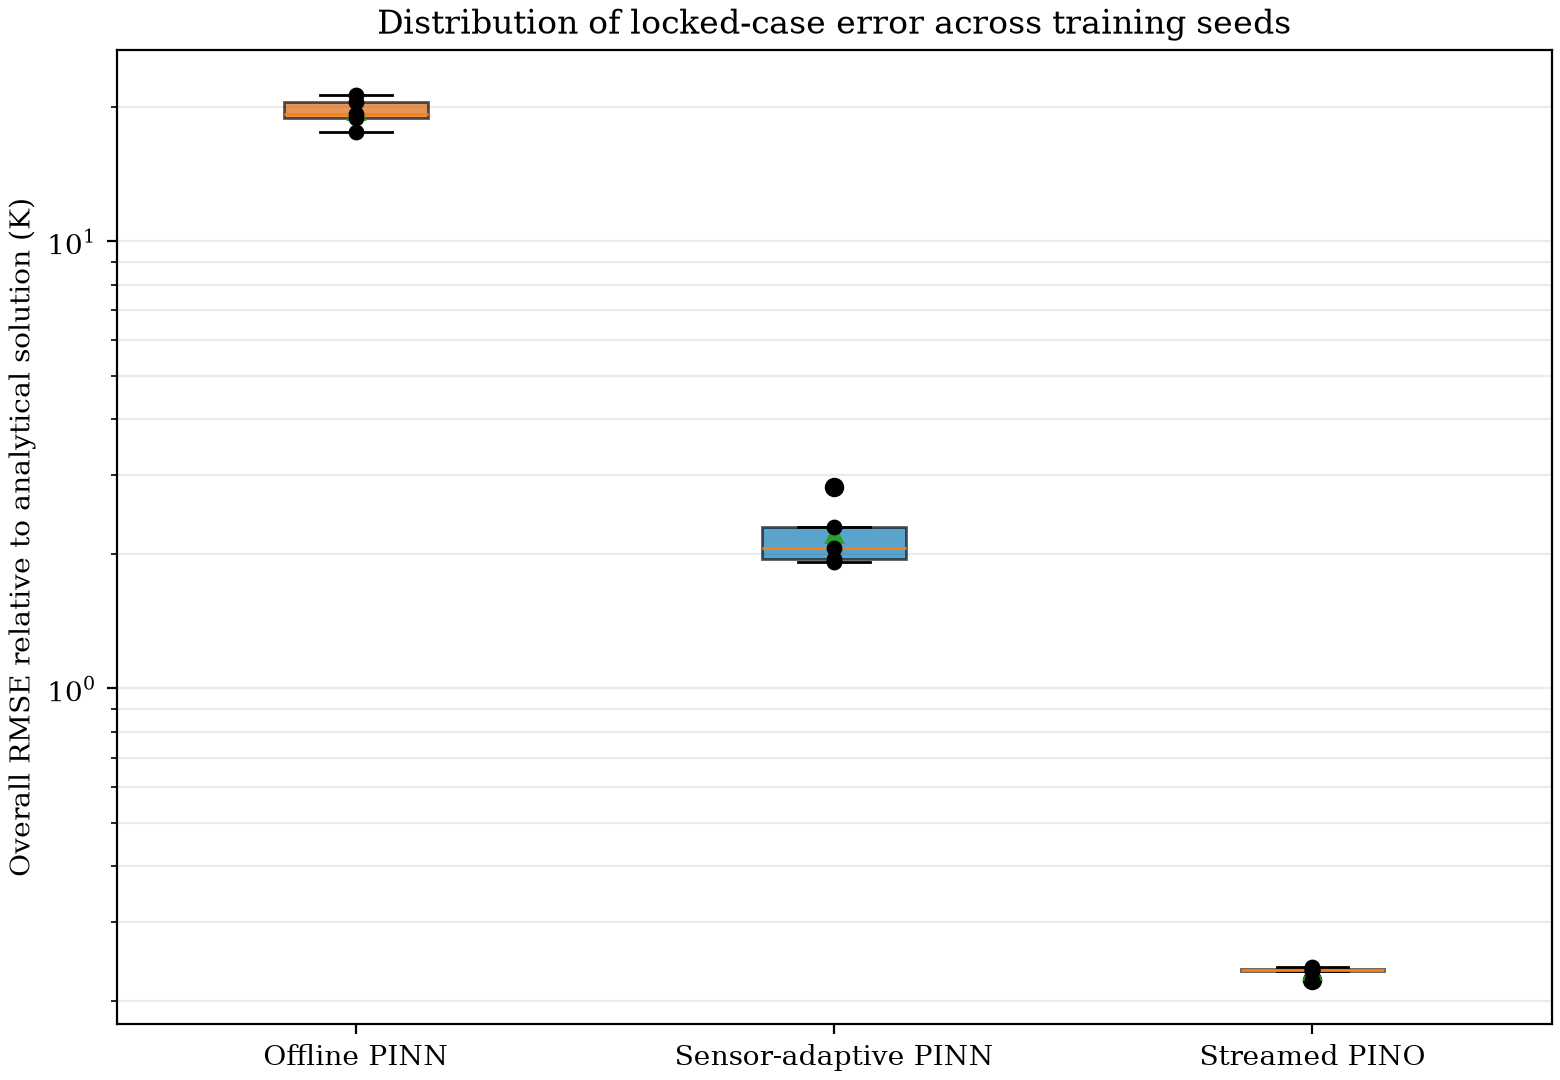
\includegraphics[width=0.82\linewidth]{locked_case_rmse_distribution.png}
  \caption{Distribution of locked-case overall RMSE across the five training seeds. Points show individual runs; boxes summarize initialization sensitivity.}
  \label{fig:latency}
\end{figure}

The latency distinction is architectural. The adaptive PINN performs gradient optimization after new measurements and requires a mean median update time of $2465\pm152$ ms. PINO performs one recurrent-state update and field decode, with mean median latency $0.862\pm0.085$ ms. Figure~\ref{fig:pinoerror} shows that locked-case, interpolation, and validation accuracy remain tightly grouped across seeds; five-seed maximum-time RMSE remains below 0.987 K.

\begin{figure}[t]
  \centering
  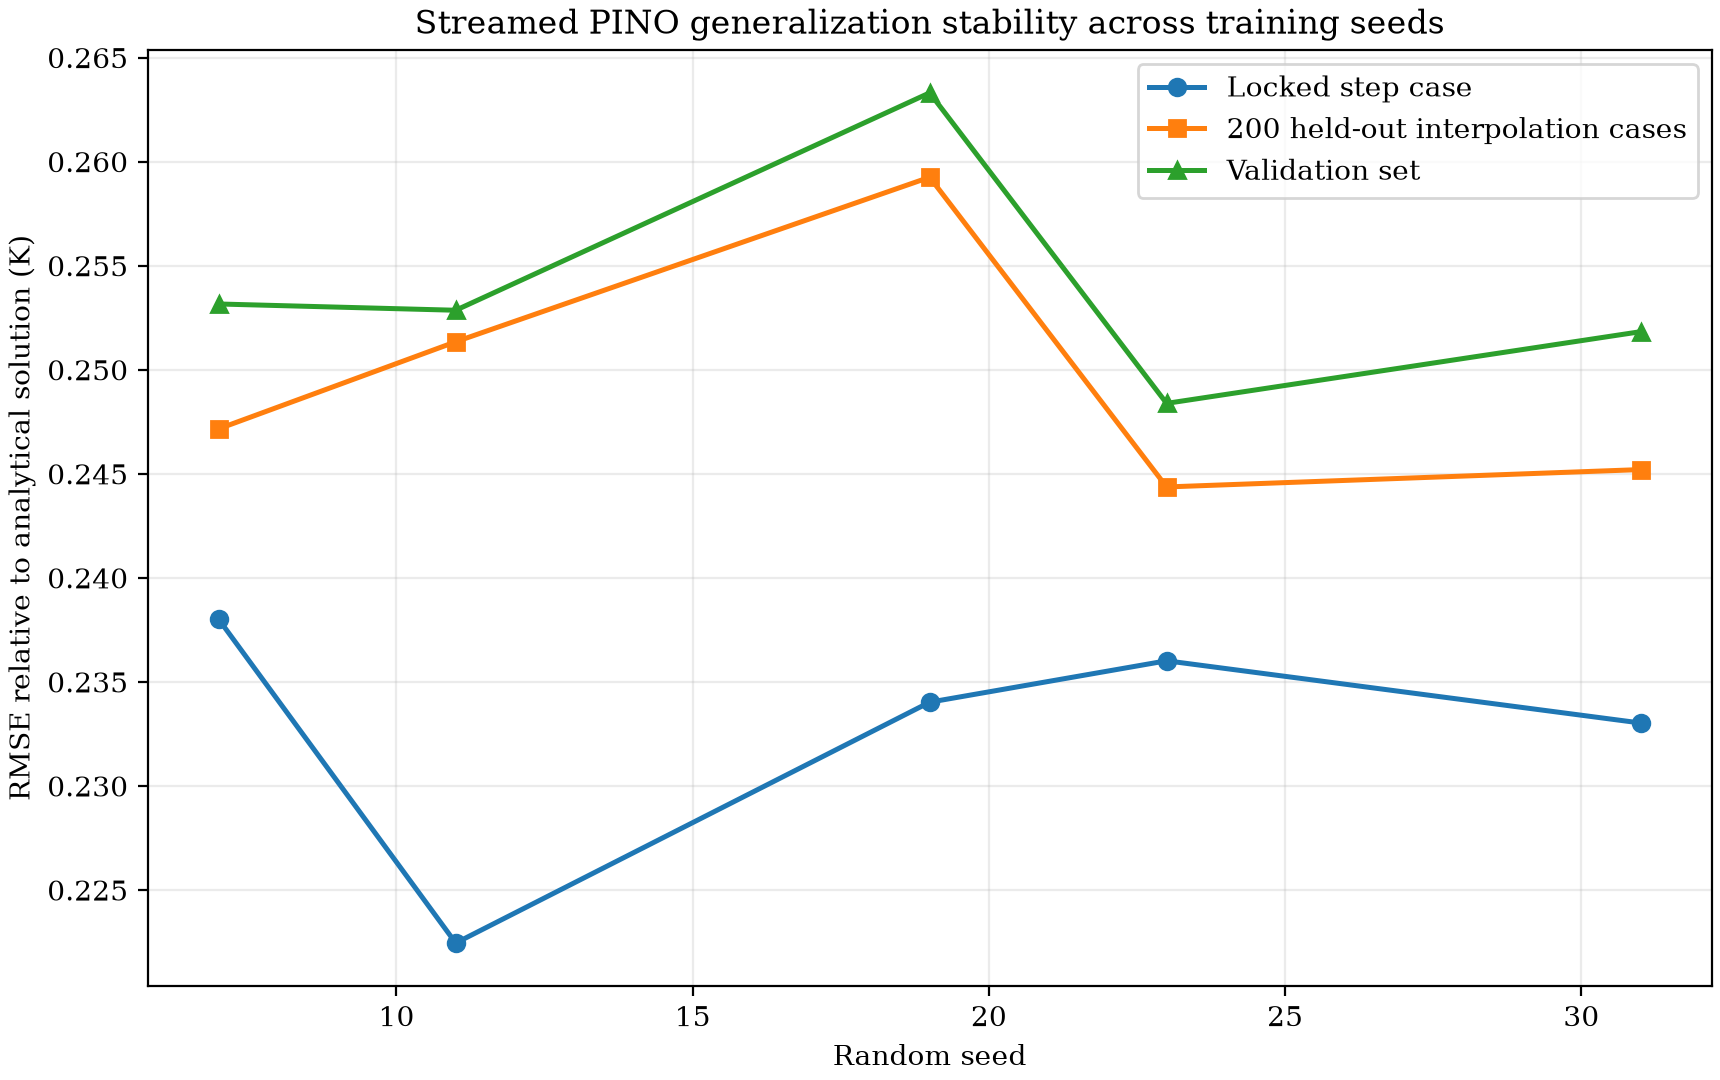
\includegraphics[width=0.78\linewidth]{pino_generalization_by_seed.png}
  \caption{Streamed-PINO generalization stability across training seeds for the locked step, 200 held-out interpolation histories, and validation corpus.}
  \label{fig:pinoerror}
\end{figure}

\subsection{Limitations}
All observations are synthetic, so the study does not include calibration error, sensor bias, uncertain properties, or geometry mismatch. Cartesian and thin-wall models neglect full nozzle curvature and conjugate coolant flow; the cylindrical reduction is accurate only when curvature variation across the wall is small. Runtime measurements are hardware-dependent. Although PINO is evaluated on 200 interpolation cases and a locked physical case across five seeds, broader extrapolation in heat flux, material properties, noise, and switch timing remains untested. The discrepancy in published Tables 2 and 3 further illustrates why reference data must be independently verified.

\section{Conclusions}
This project demonstrates an end-to-end thermal digital twin through a unified verification hierarchy. The through-thickness prototype verifies wall physics and sparse assimilation; the two-coordinate analytical benchmark verifies the extended diffusion solver and exposes a literature inconsistency. Across five seeds on a locked heat-flux change, adaptation reduces mean PINN RMSE from $19.502\pm1.441$ to $2.208\pm0.375$ K, while streamed PINO reaches $0.2327\pm0.0060$ K and sub-millisecond median latency.

The main critical insight is that online adaptation is not automatically beneficial: a sparse balanced PINN configuration degrades nominal global accuracy even though most individual updates help. Operator learning changes this tradeoff by moving expensive learning offline and maintaining only a causal observer state during operation. Future work should introduce experimental thermocouple data, uncertain properties, noise and placement sweeps, and full cylindrical or conjugate heat-transfer geometry.

\section*{Author Contributions}
Gabriel Berezovsky, Joshua Blecher, and Nathan Florsheim contributed to the physical formulation, software implementation and verification, analysis of figures and metrics, and manuscript preparation. The three-person team was completed with prior course approval.

\begin{thebibliography}{9}
\footnotesize
\bibitem{raissi2019} Raissi, M., Perdikaris, P., and Karniadakis, G. E., ``Physics-informed neural networks: A deep learning framework for solving forward and inverse problems involving nonlinear partial differential equations,'' \textit{Journal of Computational Physics}, Vol. 378, 2019, pp. 686--707. \url{https://doi.org/10.1016/j.jcp.2018.10.045}.
\bibitem{cai2021} Cai, S., Wang, Z., Wang, S., Perdikaris, P., and Karniadakis, G. E., ``Physics-Informed Neural Networks for Heat Transfer Problems,'' \textit{Journal of Heat Transfer}, Vol. 143, No. 6, 2021, 060801. \url{https://doi.org/10.1115/1.4050542}.
\bibitem{hsu2023} Hsu, H.-P., Tu, T.-W., and Chang, J.-R., ``An Analytic Solution for 2D Heat Conduction Problems with General Dirichlet Boundary Conditions,'' \textit{Axioms}, Vol. 12, No. 5, 2023, 416. \url{https://doi.org/10.3390/axioms12050416}.
\bibitem{deepxde} Lu, L., Meng, X., Mao, Z., and Karniadakis, G. E., ``DeepXDE: A Deep Learning Library for Solving Differential Equations,'' \textit{SIAM Review}, Vol. 63, No. 1, 2021, pp. 208--228. \url{https://doi.org/10.1137/19M1274067}.
\bibitem{li2021pino} Li, Z., Kovachki, N., Azizzadenesheli, K., Liu, B., Bhattacharya, K., Stuart, A., and Anandkumar, A., ``Physics-Informed Neural Operator for Learning Partial Differential Equations,'' arXiv:2111.03794, 2021. \url{https://doi.org/10.48550/arXiv.2111.03794}.
\bibitem{repository} Berezovsky, G., Blecher, J., and Florsheim, N., ``Adaptive Thermal PINN Digital Twin,'' GitHub repository, 2026. \url{https://github.com/gabebere/adaptive-thermal-pinn-digital-twin}.
\end{thebibliography}

\end{document}
